\documentclass[a4paper,15pt, oneside]{report}
\usepackage[italian]{babel}
\usepackage[utf8]{inputenc}
\usepackage[a4paper,top=2.5cm,bottom=2.5cm,left=2cm,right=2cm]{geometry}
\usepackage{amssymb}
\usepackage{amsthm}
\usepackage{graphics}
\usepackage{amsfonts}
\usepackage{amsmath}
\usepackage{amstext}
\usepackage{engrec}
\usepackage{rotating}
\usepackage[safe,extra]{tipa}
\usepackage{multirow}
\usepackage{hyperref}
\usepackage{enumerate}
\usepackage{braket}
\usepackage{marginnote}
\usepackage{pgfplots}
\usepackage{cancel}
\usepackage{polynom}
\usepackage{booktabs}
\usepackage{enumitem}
\usepackage[ruled,vlined]{algorithm2e }
\usepackage{framed}
\usepackage{pdfpages}
\usepackage{pgfplots}
\usepackage{fancyhdr}
\usepackage{caption}
\usepackage{subcaption}
\usepackage{setspace}
\usepackage{hyperref}
\usepackage{biblatex}
\usepackage{colortbl}

\usepackage{tikz}\usetikzlibrary{er}\tikzset{multi  attribute /.style={attribute
    ,double  distance =1.5pt}}\tikzset{derived  attribute /.style={attribute
    ,dashed}}\tikzset{total /.style={double  distance =1.5pt}}\tikzset{every
  entity /.style={draw=orange , fill=orange!20}}\tikzset{every  attribute
  /.style={draw=MediumPurple1, fill=MediumPurple1!20}}\tikzset{every
  relationship /.style={draw=Chartreuse2,
    fill=Chartreuse2!20}}\newcommand{\key}[1]{\underline{#1}}
\usetikzlibrary{arrows.meta}
\usetikzlibrary{decorations.markings}
\usetikzlibrary{arrows,shapes, shapes.geometric,backgrounds,petri}
\tikzset{
  place/.style={
    circle,
    thick,
    draw=black
    minimum size=6mm,
  },
  transition/.style={
    rectangle,
    thick,
    fill=black,
    minimum width=8mm,
    inner ysep=2pt
  },
  transitionv/.style={
    rectangle,
    thick,
    fill=black,
    minimum height=8mm,
    inner xsep=2pt
  }
}
\tikzset{elliptic state/.style={draw,ellipse}}

\usetikzlibrary{automata,positioning, calc}
\addbibresource{bibliography.bib}

\pagestyle{fancy}
\fancyhead[L,RO]{\slshape \rightmark}
\fancyfoot[C]{\thepage}

\title{Report della challenge di \href{http://sigmodcontest2024.eastus.cloudapp.azure.com/index.shtml}{SIGMOD}}
\author{Terzi Telemaco Matr. 865981(\href{https://github.com/Tezze2001}{@Tezze2001}) \\
        Refolli Francesco Matr. 865955(\href{https://github.com/frefolli}{@frefolli})}

\date{\today}

\pgfplotsset{compat=1.13}

\begin{document}

\maketitle

\newtheorem{teorema}{Teorema}
\newtheorem{dimostrazione}{Dimostrazione}
\newtheorem{definizione}{Definizione}
\newtheorem{esempio}{Esempio}
\newtheorem{osservazione}{Osservazione}
\newtheorem{nota}{Nota}
\newtheorem{corollario}{Corollario}
\tableofcontents
\renewcommand{\chaptermark}[1]{
  \markboth{\chaptername
    \ \thechapter.\ #1}{}}
\renewcommand{\sectionmark}[1]{\markright{\thesection.\ #1}}

\chapter{Introduzione}

Il contest di programmazione ACM SIGMOD 2024 si è articolato nello sviluppo di una soluzione 
per una variante del KNN problem (con $K=100$) per un dataset $D$ di dimensione 
$10^7$ vettori e un insieme di query $Q$ di dimensione $4\cdot 10^6$. Ciascun 
vettore del dataset possiede dei metadati che specificano la sua categoria e il
suo timestamp. Dal momento che si hanno dei metadati associati ai vettori, si 
identificano anche $4$ tipologie, ognuna specifica dei filtri da applicare sui 
metadati del dataset:
\begin{itemize}
    \item Query tipo $0$: non si applicano filtri sui metadati.
    \item Query tipo $1$: si filtra il database rispetto alla categoria specificata della query, si considerano 
    solo i vettori che hanno la stessa categoria del vettore di query.
    \item Query tipo $2$: si filtra rispetto all'intervallo di timestamp specificato della query,
    si considerano solo i vettori che hanno il timestamp compreso nell'intervallo 
    specificato dal vettore di query.
    \item query tipo $3$: si applicano entrambi i filtri della tipologia $1$ e $2$.
\end{itemize}

I vettori di query e del dataset, oltre ai metadati, hanno associato anche le $100$ 
componenti su cui calcolare il concetto di vicinanza.

Il codice della risoluzione verrà testato in una macchina virtuale con $32$ Thread,
$64Gb$ di RAM e $64Gb$ di spazio. Si ha inoltre un tempo massimo di esecuzione 
di $20$ minuti.

Formalmente, il problema introdotto precedentemente può essere descritto nel 
seguente modo. Siano $D\subseteq \mathbb{R}^{100}$ e $Q\subseteq \mathbb{R}^{100}$
rispettivamente gli insiemi dei vettori di dataset e del queryset.

Siano $c:D\cup Q\to \mathbb{N}$ e $t:D\to \mathbb{R}_+$ le funzioni che restituiscono 
la categoria e il timestamp dei vettori del dataset e/o del queryset.
Sia $type: Q\to \{0, 1, 2, 3\}$ e $bound:Q \to \mathbb{R}^2_+$ le funzioni
che restituiscono rispettivamente la tipologia e l'intervallo di timestamp dei 
vettori del queryset.

Quindi la ricerca si effettua in base ai casi, $\forall q\in Q$:
\begin{itemize}
    \item $type(q) = 0$ (query senza filtraggio): si cerca $S_q$ ($S_q \subseteq D$ 
    e $|S_q| = 100$) tale che 
    $$\forall s \in S_q, d(s, q) \le d(x, q) \forall x \in D \setminus S_q$$  
    \item $type(q) = 1$ (query filtrando sulla categoria): si cerca $S_q$ ($S_q \subseteq \{x| x\in D, c(x) = c(q)\}$ 
    e $|S_q| = 100$) tale che 
    $$\forall s \in S_q, d(s, q) \le d(x, q) \forall x \in \{x| x\in D \setminus S_q, c(x) = c(q)\}$$  
    \item $type(q) = 2$ (query filtrando sull'intervallo di timestamp): si cerca 
    $S_q$ ($S_q \subseteq \{x| x\in D, t(x) \in timestamp(q)\}$ 
    e $|S_q| = 100$) tale che 
    $$\forall s \in S_q, d(s, q) \le d(x, q) \forall x \in \{x| x\in D \setminus S_q, t(x) \in timestamp(q)\}$$  
    \item $type(q) = 3$ (query filtrando sull'intervallo di timestamp e sulla categoria): si cerca 
    $S_q$ ($S_q \subseteq \{x| x\in D, t(x) \in timestamp(q),  c(x) = c(q)\}$ 
    e $|S_q| = 100$) tale che 
    $$\forall s \in S_q, d(s, q) \le d(x, q) \forall x \in \{x| x\in D \setminus S_q, t(x) \in timestamp(q), c(x) = c(q)\}$$  
\end{itemize}
Dove $d$ è la distanza euclidea applicata alle $100$ componenti dei vettori.
 
La soluzione finale $\mathcal{S}$ coinciderà con $ \mathcal{S} = \bigcup_{q\in Q} S_q$.

\section{Approcci tentati}
Un modo per risolvere questo problema è adottare l'approccio naive esaustivo (EN), ovvero 
confrontare ciascun vettore di query con tutti i vettori del database filtrato. 
A livello di complessità è insostenibile, infatti supponento nel caso peggiore 
di avere solo query del tipo $0$, significa che si calcoleranno un totale di 
$\mathcal{O}(|Q| \cdot |D|)$ distanze, con l'aggiunta della complessità di creazione
della soluzione. La creazione della soluzione può essere trattata mediante l'ausilio 
di un max-heap, contenente le coppie vettore database e distanza vettore-2-query ($D\times \mathbb{R}_+$),
la dimensione può essere considerata fissa a $K(=100)$, questo significa che l'inserimento 
della singola coppia comporta una complessità $\mathcal{O}(K)$. Dal momento che 
si tenterà di inserire $\mathcal{O}(|D|)$ coppie allora la costruzione della 
soluzione per ogni singola query sarà $\mathcal{O}(|D|\cdot K)$, complessivamente per l'intero 
queryset si avrà $\mathcal{O}(|Q| \cdot |D|\cdot K)$. Dal momento che $K$ è costante 
a $100$ allora si può approssimare la complessità di costruzione della soluzione 
a  $\mathcal{O}(|Q| \cdot |D|)$. Complessità che risultano essere proibitive quando 
si lavora su $|D|= 10^7$ e $|Q|= 4\cdot 10^6$, infatti supponendo di impiegare $1ms$ 
a calcolare una singola distanza allora significa che per effettuare solo tutti i 
confronti si impiegherà $0,001 \cdot |D| \cdot |Q| = 4\cdot 10^{10}$
secondi che vuol dire circa $1268$ giorni, anche parallelizzando al massimo 
il tutto si impiegherà circa $1268/32 = 39$ giorni. 

EN non può essere adottata come soluzione finale, ma è stata utile per poter 
stimare la Recall dei metodi sviluppati in seguito. Infatti, dal momento che i 
creatori della challenge hanno rilasciato differenti versioni del dataset ($10^4, 10^6, 10^7$) e del 
queryset ($10^2, 10^5, 10^6$), è stato possibile confrontare le soluzioni di EN
e dei metodi sviluppati sui dataset con una grandezza minore. 

Visto che EN è proibitivo, è stata effettuata una ricerca sulla letteratura 
relativa all'argomento. Da questa ricerca sono stati estratti diversi approci, 
un primo approccio si basa sull'uso di alberi metrici come \textbf{KD-tree} \cite{kd_tree}, \textbf{MVP-tree}
\cite{mvp_tree1} \cite{mvp_tree2}, \textbf{VP-tree} \cite{vp_tree} e \textbf{Ball-tree} \cite{ball_tree}
che funzionano bene per vettori che hanno una dimensione ridotta, ma esplodono 
di complessità quando vengono eseguiti su dimensioni elevate come nell'attuale 
caso in esame. Perciò è stato pensato di applicare i metodi dopo aver applicato 
un algoritmo di riduzione di dimensionalità con l'obiettivo di ridurre 
i tempi di esecuzione.

Sono stati testati gli algoritmi di riduzione come \textbf{Principal Component Analysis} (PCA) \cite{pca}
e \textbf{Random Projection} (RP) \cite{rp}. PCA è stato immediatamente scartato dal momento che 
calcolando la matrice di correlazione sul dataset $D$ si è ottenuta un'assenza 
di correlazione tra le componenti che preannuncia una spiegazione di variabilità 
di dati uniforme tra tutti gli autovettori della matrice di correlazione, comportando 
una mancanza di componenti con maggior information gain. Perciò è stato provato 
un approccio alternativo con Random Projection (RP) che ha permesso di ridurre la 
dimensionalità a $90$ componenti per preservare la recall sopra il $90\%$, ma 
senza significativi miglioramenti nei tempi di esecuzione degli alberi metrici.

Successivamente è stato tentato l'approccio dei grafi metrici come \textbf{Hierarchical 
Navigable Small World Graphs} (HNSW) \cite{hnsw}. A livello teorico permette di ridurre i tempi
di ricerca (infatti la complessità è $\mathcal{O}(log |D|)$), il problema è 
che la costruzione della struttura è risutata troppo pesante e non è stato trovato 
un modo per migliorare i tempi. Il problema principale della costruzione è 
il fatto che alla fine si va a calcolare un totale di $\mathcal{O}(|D|\cdot |D|)$
distanze che a livello di tempo è risultato proibitivo.

Successivamente è stato tentato l'approccio della quantizzazione dei vettori con 
la \textbf{Product Quantization} (PQ) \cite{pq} e gli \textbf{Inverted File Index} (IVF)\cite{pq}. Il problema di questi 
due approcci è che richiedono troppo tempo per costruire l'indice dal momento che 
PQ nasconde $M(=10)$ Kmeans ($K=256$ cluster l'uno) che eseguiti in parallelo si 
è riusciti a mantenere contenuti i tempi di costruzione, ma con una Recall troppo 
bassa ($\sim 0.6$). Invece, IVF nasconde prima un Kmeans con più di $1024$ cluster 
e poi una PQ con $M(=10)$ Kmeans ($256$ cluster l'uno), ottenendo una recall simile 
a PQ, ma con tempi maggiorati a confronto. 

Per ridurre i tempi è necessario ridurre i centroidi comportando un aumento dell'errore 
di quantizzazioen dei vettori e peggiorando, di conseguenza, la Recall.

Infine è stata trovato l'approccio finale basato su $LSH$ che ha permesso, attraverso 
una fase di fine-tuning dei parametri, di raggiungere un compromesso tra tempi di 
esecuzione e Recall discreti.









\chapter{Soluzione proposta}
L'approccio vincente si è basato su \textbf{locality-sensitive hashing} (LSH).
Gli approcci basati su LSH consistono nella definizione di una funzione di hash 
che ha l'obiettivo di partizionare il dataset $D$ in una hash table composta 
da una serie di bucket, ciascuno 
formato in modo tale da contenere vettori che sono i più simili possibili, rispetto 
alla distanza euclidea. 

La costruzione della funzione di hash deve essere fatta in modo tale da 
massimizzare il numero di collisioni tra i vettori simili e ridurre al minimo 
il numero di collisioni per vettori differenti. 

In questo modo la ricerca si articola in:
\begin{itemize}
    \item calcolare l'hash della query che definisce l'indice del bucket
    \item calcolare le distanze tra la query e tutti i vettori nel bucket ed 
    estrarre i 100 più vicini
\end{itemize} 

Questo approccio permette di ridurre il numero di distanze calcolate, dal momento 
che si confrontano solo la query con i vettori nel bucket. Il problema è trovare 
un approccio per costruire una funzione di hash che sia veloce da calcolare e 
che permetta di creare dei bucket di buona qualità.

\section{Costruzione della funzione di hash}

La funzione di hash che è stata definita si basa su \textbf{Random Projection}(RP),
esattamente lo stesso algoritmo di riduzione di dimensionalità. 

L'idea è di definire $k' = \lceil \log_2{\sqrt{|D|}} + 2\rceil (= 14)$  iperpiani randomici che suddividono
lo spazio dei vettori del dataset in $2^{k'}$ regioni, ad ogni regione si associa 
un hash e tutti i vettori che cadono afferiscono alla stessa regione produrranno 
una collisione, quindi verranno inseriti nello stesso bucket.

\begin{nota}
    La formula per ottenere $k'$ è stata scelta in modo arbitrario basandosi sulle 
    sugli studi empirici e suoi risultati ottenuti in termini di Recall e tempi
    di esecuzione.
\end{nota}

Ogni singolo $i$-esimo iperpiano è stato definito dal suo vettore norma $n_i$,
generato randomicamente estraendo le singole componenti da una distribuzione uniforme 
($n_i \in U[-1,1]^{100}$). L'hash di un vettore viene calcolato considerandolo 
come un numero binario di $k'$ bit, dove l'$i$-esimo bit $h_i$ dell'hash specifica:
\begin{itemize}
    \item $h_i = 1$: il vettore $v$ si trova sopra L'iperpiano definito dalla 
    norma $n_i$
    \item $h_i = 0$: il vettore $v$ si trova sotto L'iperpiano definito dalla 
    norma $n_i$
\end{itemize}

A livello matematico si riduce all'equazione 
$$h_i = \begin{cases}
    1 & n_i \cdot v \ge 0\\
    0 & n_i \cdot v < 0
\end{cases}$$ 

Dove $\cdot$ è il prodotto interno in $\mathbb{R}^{100}$. Lo pseudocodice della 
funzione di hash è stato riportato nel listato \ref{list:funzione_hash}.

\begin{algorithm}
    \SetAlgoLined
    \KwData{vettore $v\in D$}
    \KwResult{hash $h\in \mathbb{N}$}

    \Begin{
        $h= 0$\;
        \For{$i=1$ \KwTo $k'$}{
            $partial = n_i \cdot v$\;
            $h = h << 1$\;
            \If{$partial \ge 0$}{
                $h= h+1$\;
            }
        }
    }
    \caption{Pseudocodice della funzione di hash.}
    \label{list:funzione_hash}
\end{algorithm}

\begin{nota}
    L'hash viene calcolato solo sulle componenti del vettore e non sui metadati.
\end{nota}

La complessità temporale della funzione di hash calcolata per un particolare $v\in V$,
è $\mathcal{O}(k' \cdot |v|)$ dove 
$|v|$ è il numero delle componenti di $v\in D$ che dai requisiti della challenge 
costante a $100$, perciò si può anche approssimare a $\mathcal{O}(k')$, ma essendo 
che anche $k'$ è costante allora si piò approssimare a $\mathcal{O}(1)$.

\section{Costruzione di LSH}

La struttura dati di LSH dovrà contenere l'hash table dei vettori e le norme degli 
iperpiani generati.
Nella realtà viene salvato anche il mapping inverso dal vettore del dataset al 
suo hash associato.

La costruzione della struttura si articola in tre passi:
\begin{itemize}
    \item calcolo dell'hash per ogni vettore del dataset e salvataggio del mapping 
    vettore-hash
    \item creazione dei bucket e inserimento dei vettori
    \item ordinamento dei vettori nei bucket
\end{itemize}

Il calcolo dell'hash viene effettuato per ogni vettore e si salva il risultato 
all'interno di un array $v_h$:

$$v_h[i] = h(v_i)$$

Successivamente si costruiscono i bucket $M_h$, a livello implementativo ciascun bucket 
è una \texttt{unordered\_map}, che coincidono con 

$$M_h = \{v\in D : h = h(v)\}$$

\begin{nota}
    La scelta di utilizzare \texttt{unordered\_map} piuttosto che \texttt{map} è dovuta ai tempi di 
    accesso e ricerca degli elementi:
    \begin{itemize}
        \item \texttt{unordered\_map}: il tempo di accesso usando l'hash è costante 
        nel caso medio e lineare nel caso peggiore, inoltre il tempo di ottenimento dell'hash 
        dato un vettore è costante nel caso medio e lineare nel caso peggiore. \cite{unsorted_map_index}\cite{unsorted_map_find}
        \item \texttt{map}: il tempo di accesso usando l'hash è logaritmico nella dimensione 
        del container, mentre il tempo di ottenimento dell'hash dato un vettore è
        logaritmico. \cite{map_index}\cite{map_find}
    \end{itemize}
\end{nota}

Per ultimo si effettua un ordinamento dei vettori nei singoli bucket, più precisamente
si ordina prima timestamp e successivamente per le componenti dei vettori.

I tempi di costruzione della struttura coincidono con $\mathcal{O}(|D|\cdot 1)$
per il mapping vettore-hash, $\mathcal{O}(|D|\cdot |D|)$ ($\Theta(|D|)$) per l'inserimento 
dei vettori nei bucket e $\mathcal{O}(|D|\log |D|)$ per l'ordinamento dei vettori 

Parlando invece dello spazio occupato, la struttura ha una complessità spaziale 
limitata perché non si salvano completamente i vettori in ciascuna sottostuttura,
bensì si salvano i loro indici di posizione del dataset, in aggiunta gli hash non 
sono altro che interi. Quindi il vettore di mapping vettori-hash $v_h$ alla fine 
contiene un totale $|D|$ interi, mentre l'unsorted map conterrà sempre gli indici 
dei vettori, in totale $|D|$, e tutti gli hash, quindi al massimo $2^{k'} = 2^ {14}$ 
interi, infine complessivamente si ha un totale di al massimo $10^7 + 2^{14}$ interi 
da salvare ($\approx 38 Mb$).

Il problema di questa soluzione è la Recall che è risultata bassa fin da subito, 
in fatti uno dei problemi e allo stesso tempo pregi di questo metodo è che la ricerca 
dei vettori più vicini si effettua solo nel bucket in cui cade il vettore di query.
Questo permette di ridurre il numero di distanze calcolate per ogni query, ma non 
considera anche vettori vicini alla query che fanno parte di bucket adiacenti.

\begin{esempio}
    Se i dati sono molto densi in alcune regioni del piano e sparsi in altre c'\`e la possibilit\`a
    che un gruppo denso di punti sia diviso in pi\`u bucket limitando la nostra capacit\`a di leggere tutti
    i vettori "realmente" vicini a quello di query.
\end{esempio}

\begin{esempio}
    Possiamo aver problemi anche nel caso generale in cui la query sia di tipo $0$, quindi non si 
    deve filtrare per metadati, e cade nello spazio vicino ad un iperpiano che limita il bucket, 
    questo comporta che in fase di ricerca si consideranno solo i vettori di quel 
    bucket e non quelli del bucket adiacente che ha in comune lo stesso iperpiano. 
\end{esempio}

Per risolvere i problemi è stato pensato di generare nuovi mapping randomici (\textbf{LSH con hash table multiple})

\section{LSH con hash table multiple}

Precedentemente è stato introdotto LSH composta da una hash table che mappa i vettori 
in bucket identificati dal loro hash.

L'idea di LSH con hash table multiple è di creare un totale di $M$ hash table ognuna con un
inizializzazione tramite iperpiani il più differente possibile dalle altre. In questo 
modo è possibile suddividere l'intero spazio dei vettori in $M$ modi differenti,
cosicché in fase di ricerca, al posto che cercare in una hash table, si cerca 
in $M$ hash table parallelamente. In questo modo si può considerare anche alcuni vettori che ricadrebbero in bucket vicini,
perché si spera che i bucket in cui cade la query per ciascuna hash table siano composti da vettori diversi.
$M$ è stato scelto attraverso uno studio sull'impatto dei parametri sulle sulle metriche di tempo (di costruzione e ricerca) e recall.

La differenza di partizione dello spazio di ciascuna hash table dipende interamente 
da come vengono generati gli iperpiani di separazione, dal momento che si estraggono 
da una distribuzione uniforme si ha già una buona variabilità e questo permette di avere 
una maggior variabilità anche nelle hash table, portando a dei miglioramenti in termini di 
recall.

Bisogna però menzionare il fatto che le diverse hash table partizionano lo stesso 
spazio geometrico, quindi in fase di ricerca può capitare che la query venga confrontata 
più volte con gli stessi vettori perché questi, essendo vicini, possono capitare 
negli stessi bucket della query in hash table differenti.

Quindi introducendo $M$ hash table multiple, significa che si effettueranno $M$ 
diverse separazioni dello spazio dei vettori del dataset, perciò si avranno 
$M$ diversi insiemi di norme e perciò il calcolo dell'hash per ciascuna hash table 
si basa sull'insieme di norme associate alla medesima hash table.

Visto che l'introduzione di hash table multiple può portare a confronti multipli 
tra la query e gli stessi vettori, per ridurre i tempi di ricerca e aumentare 
la recall sulle query di tipo $1$ e di tipo $3$ è stato pensato di definire una 
\textbf{LSH Forest}.

\section{Esplorazione dei Bucket Adiacenti}

Si \`e anche pensato alla possibilit\`a di identificare a runtime i bucket adiacenti a quello della query per esplorarli e migliorare la recall, come alternativa ad avere pi\`u hash tables.
Questa operazione pu\`o essere fatta semplicemente considerando la \textbf{distanza di hamming} di due hash: con $HD = 1$ i due hash differiranno del posizionamento rispetto ad un iperpiano, di conseguenza esplorando tutti gli hash con questa distanzia stiamo visitando gli spazi adiacenti. Questo corrisponde ad effetturare uno xor dell'hash con $k$ bitmask del tipo $0^i10^j$, con $i + j + 1 = k$.
Il problema principale di questa strategia non \`e nella sua implementazione quanto nel fatto che rappresenta un'ennesima euristica basata sulla fortuna: se un query viene mappato in un bucket con pochi vettori e poi esplorando gli adiacenti ci imbattessimo in un bucket con molti vettori andremmo a peggiorare notevolmente l'esecuzione senza avere la certezza di trovare pi\`u vicini.
Sperimentalmente si \`e rilevato che l'aumento di recall \`e relativamente insignificante e che viceversa l'aumento dei tempi di ricerca peggiora nel complesso la qualit\`a della soluzione.

\section{LSH Forest}
L'approccio di LSH Forest è di velocizzare le query che filtrano sulla categoria,
ovvero quelle di tipo $1$ e $3$. Per fare ciò è stato pensato di definire una \textbf{LSH
con hash table multiple generale} sull'intero dataset per le query di tipo $0$ e $2$ e definire,
per ogni categoria sufficientemente grande ($>2000$), una \textbf{LSH con hash table multiple}, in questo 
modo si riduce il numero di distanze calcolate. La scelta di creare 
una LSH dedicata solo per le categorie che superano la cardinalità dei $2000$ vettori 
è dovuta dal fatto che il tempo necessario per crearla è maggiore dei benefici 
che porta nella ricerca, quindi si preferisce evitare di crearla.

L'unico problema che rimane da risolvere in fase di costruzione di LSH Forest è 
indentificare i vettori della stessa categoria nel dataset, per fare ciò è bastato 
ordinare il dataset dei vettori secondo la categoria, il timestamp ed infine 
le componenti di ciascun vettore. Questo richiede $\mathcal{O}(|D|\log |D|)$ di 
complessità, ma non aggiunge complessità alla costruzione delle LSH per ogni categoria 
dal momento che i vettori della stessa categoria sono tutti continui. Questa 
fase di ordinamento, inoltre, velocizza l'ordinamento dei vettori nei bucket e la ricerca 
filtrando per il timestamp. L'ordinamento dei vettori del bucket non è detto 
che venga preservato perché la costruzione è parallelizzata.

Quindi ricapitolando la costruzione si articola nelle seguenti fasi:
\begin{itemize}
    \item \textbf{ordinamento del dataset} secondo la categoria, timestamp e componenti dei vettori.
    \item \textbf{indicizzazione delle categorie}: creazione di una mappa che 
    associa a ciascuna categoria una tupla che specifica gli indici 
    del primo e dell'ultimo vettore nel dataset di quella categoria.
    \item \textbf{creazione di LSH con hash table multiple} sull'intero dataset.
    \item \textbf{creazione di una LSH con hash table multiple} per ogni categoria 
    di dimensione maggiore di $2000$ vettori.
\end{itemize}

L'algoritmo finale di costruzione di LSH Forest è mostrato nel listato \ref{list:costruzione_lsh_forest}.

\begin{algorithm} [!h]
    \SetAlgoLined
    \KwData{dataset $D$}
    \KwResult{LSH Forest $LSHF$}
    
    \Begin{
        $sort(D)$\;
        $c\_map = index(D)$\;
        $LSHF.general = createLsh(D,0,|D| - 1)$\;
        \For{$\forall c\in C$}{
            \If{$c\_map[c].end - c\_map[c].start > 2000$}{
                $lsh = createLsh(D,c\_map[c].start,c\_map[c].end)$\;
            }{
                $lsh = Null$\;
            }
            $LSHF.mapped[c] = lsh$\;
        }
    }

    
    \SetKwFunction{FLsh}{createLsh}
    \SetKwProg{Fn}{Function}{:}{}
    \Fn{\FLsh{$D$, $start\_idx\_cat$, $end\_idx\_cat$}}{
        \Begin{
            $lsh$ is object\;
            $length =end\_idx\_cat - start\_idx\_cat$\;
            \For{$i=1$ \KwTo $NHashTable$}{
                $hp = generateHyperplanes()$\;
                $lsh.hashtable[i].hp = hp$\;
                $hashes$ is array\;
                \For{$j=1$ \KwTo $|length|$}{
                    \For{$k=1$ \KwTo $|hp|$}{
                        $hashes[j] = hash(hp[k], D[start\_idx\_cat + j])$\;
                    }
                }
                $lsh.hashtable[i].hashes = hashes$\;
                \For{$j=1$ \KwTo $|D|$}{
                    $lsh.hashtable[i].buckets[hashes[j]].push(start\_idx\_cat + j)$\;
                }

                \For{$j=1$ \KwTo $|hp|$}{
                    $sort(lsh.hashtable[i].buckets[j])$\;
                }
            }
            \Return{$lsh$}
        }
    }

    \caption{Pseudocodice della costruzione di LSH Forest. La funzione $index$ genera 
    una mappa che associa ad ogni categoria la posizione di inizio e di fine del 
    gruppo di vettori che afferisce alla stessa categoria. La funzione 
    $generateHyperplanes$ ritorna l'array delle norme degli iperpiani generate 
    randomicamente.}
    \label{list:costruzione_lsh_forest}
\end{algorithm}

La complessità di creazione di LSH Forest può essere riassunta in:
\begin{itemize}
    \item \textbf{ordinamento del dataset}: $\mathcal{O}(|D|\log |D|)$
    \item \textbf{indicizzazione delle categorie}: $\mathcal{O}(|D|)$
    \item \textbf{creazione di LSH con hash table multiple} generale: la generazione
    di una hash table richiede $\mathcal{O}(k'\cdot |v|=1)$ per generare gli iperpiani
    (dove $|v| = 100, k' = 14$), $\mathcal{O}(|D|\cdot 1)$ per calcolare l'hash per ogni vettore,
    $\mathcal{O}(|D|)$ per inserire i vettori nei bucket e infine $\mathcal{O}(|D|\log |D|)$
    per ordinare tutti i bucket. Queste operazioni si devono replicare per tutte le 
    $M$ hash table quindi in totale si impiegherà $\mathcal{O}(M\cdot |D|\log |D|)$.
    Da notare che i bucket potenzialmente sono già parzialmente ordinati quindi 
    l'ordinamento a livello asintotico si avvicina a $\mathcal(|D|)$ e quindi 
    potenzialmente la complessità della creazione di tutte le hash table è $\mathcal{O}(M\cdot |D|)$.
    \item \textbf{creazione di una LSH con hash table multiple} per ogni categoria 
    di dimensione maggiore di $2000$ vettori: per la creazione di ciascuna LSH 
    è, come detto precedentemente, vicino a $\mathcal{O}(M\cdot |c|)$ dove $|c|$
    è la dimensione della categoria.
\end{itemize}

In realtà la costruzione viene ottimizzata parallelizzando la costruzione delle 
singole LSH.

\section{Ricerca in LSH Forest}

La ricerca nella struttura cambia in base alla tipologia di query che si deve 
cercare:
\begin{itemize}
    \item query senza filtraggio e query con il filtraggio sul timestamp: la ricerca 
    si effettua solo nell'LSH generale contenente tutti i vettori.
    \item query con il filtraggio sulla categoria e query con il filtraggio sulla 
    categoria e timestamp: la ricerca si effettua in modo esaustivo nel dataset per quelle 
    categorie con meno di $2000$ vettori, altrimenti per le altre si ricerca 
    nella LSH della categoria. 
\end{itemize}

Per ogni query si produce un Minheap contenente le $100$ migliori coppie 
$(idx_v, d(v,q))$, ovvero indice del vettore $v$ nel dataset e distanza tra il vettore
e la query. Il Minheap deve ordinare rispetto la distanza.

La ricerca di una \textbf{query senza filtraggio o query con filtraggio sul timestamp} 
si effettua nell'LSH generale costruita sull'intero dataset. Più precisamente la 
query senza filtraggio si ricerca nel seguente modo, per ogni hash table 
delle $20$ si estraggono i vettori a distanza minima dalla query e poi si combinano 
i risultati. Più precisamente, per ogni $i$-esima hash table:
\begin{itemize}
    \item si calcola $h_i(q)$
    \item si cerca il bucket di vettori che sono mappati con il medesimo hash 
    di $h_i(q)$
    \item si calcolano le distanze tra i vettori del bucket e la query e si inseriscono
    nel Minheap
\end{itemize}
Per il caso delle query con filtraggio sul timestamp si effettuano i seguenti passi,
per ogni $i$-esima hash table:
\begin{itemize}
    \item si calcola $h_i(q)$
    \item si cerca il bucket di vettori che sono mappati con il medesimo hash 
    di $h_i(q)$
    \item si effettua una ricerca dicotomica nel bucket degli indici di due vettori: quello con 
    il minimo timestamp che è maggiore di $q.l$ e quello col massimo timestamp che 
    è minore di $q.r$. In questo modo si trova il intervallo di vettori nel bucket 
    che hanno timestamp compreso tra $[l,r]$.
    \item si calcolano le distanze tra i vettori del bucket e la query e si inseriscono
    nel Minheap
\end{itemize}

La ricerca di una \textbf{query con filtraggio solo sulla categoria o sulla categoria e timestamp}, 
per categorie piccole $|c|\le 2000$, viene effettuata in modo esaustivo direttamente nel dataset,
sfruttando il suo ordinamento e l'indicizzazione della $c\_map$ costruita 
prima di creare $LSHForest$. 
Più precisamente, dal momento che il dataset viene ordinato, da $c\_map[c]$
si ottiene $[idx_l, idx_r]$, l'intervallo vettori afferenti alla stessa categoria della query. 
Se la query filtra solo per categoria si calcolano le distanze tra la query e tutti 
i vettori della regione, popolando di conseguenza il minheap. 
Nel caso in cui la query filtra anche per timestamp, 
dal momento che la regione è anche ordinata per timestamp, allora si effettua 
una ricerca dicotomica degli indici di due vettori: quello con il minimo timestamp che è 
maggiore di $q.l$ e quello col massimo timestamp che è minore di $q.r$.
In questo modo si ottiene un intervallo 
di indici dei vettori nel dataset che hanno timestamp incluso 
nell'intervallo specificato dalla query. Infine si calcolano tutte le distanze 
tra i vettori dell'intervallo e la query, popolando alla fine il minheap.

Per le medesime query, ma sulle categorie più grandi $|c|> 200$ allora la ricerca 
si effettua direttamente nelle LSH dedicate della categoria con lo stesso algoritmo 
spiegato per la ricerca delle query senza filtraggio o query con filtraggio sul timestamp.

Lo pseudocodice è mostrato nel listato \ref{list:ricerca_lsh_forest}.



\begin{algorithm} [!h]
    \SetAlgoLined
    \KwData{dataset $D$, $LSHF$ e query $q$}
    \KwResult{vettori $K \subseteq D$}
    
    \Begin{
        \Switch{query.type}{
            \Case{$query.type == 0 \lor query.type == 2$}{
                \Return{$searchLsh(LSHF.general, D, q)$}
            }
            \Case{$query.type == 1\lor query.type == 3$}{
                \If{$LSHF.mapped[c].hashtable != null$}{
                    \Return{$searchLsh(LSHF.mapped[c],D, q)$}
                }\Else{
                    \Return{$ExaustiveSearch(D, q)$}
                }
            }
        }
    }

    \SetKwFunction{FLsh}{searchLsh}
    \SetKwProg{Fn}{Function}{:}{}
    \Fn{\FLsh{$LSH$,$D$, $q$}}{
        \Begin{
            $results$ is a Minheap\;
            \Switch{$q.type$}{
                \Case{$q.type == 2 \lor q.type == 3$}{
                    \For{$i=1$ \KwTo $Ns$}{
                        $h_q = hash(LSH.hashtable[i],q)$\;
                        $bucket = LSH.hashtable[i].bucket[h_q]$\;
                        $[idx_l, idx_r] = dicotomicSearch(D, bucket, q.l, q.r)$\;

                        \For{$v\in D[idx_l:idx_r]$}{
                            \If{$\lnot results.has(v)$}{
                                $results.insert((idx(v), distance(v,q)))$\;
                            }                            
                        }
                        \Return{$lsh$}
                    }

                }
                \Case{$q.type == 0 \lor q.type == 1$}{
                    \For{$i=1$ \KwTo $NHashTable$}{
                        $h_q = hash(LSH.hashtable[i],q)$\;
                        $bucket = LSH.hashtable[i].bucket[h_q]$\;
                        $[idx_l, idx_r] = dicotomicSearch(D, bucket, q.l, q.r)$\;

                        \For{$idx\in bucket$}{
                            \If{$\lnot results.has(v)$}{
                                $results.insert((idx, distance(D[idx],q)))$\;
                            }              
                        }
                        \Return{$lsh$}
                    }

                }
            }
            
        }
    }

    \caption{Pseudocodice per la ricerca della query in LSH Forest.}
    \label{list:ricerca_lsh_forest}
\end{algorithm}

La complessità della ricerca varia in base alle query che si devono cercare e dalla 
composizione del dataset:
\begin{itemize}
    \item \textbf{query senza filtraggio}: il calcolo dell'hash è approssimato a $\mathcal{O}(1)$,
    trovare il bucket con lo stesso hash è $\mathcal{O}(|D|)$ (costante nel caso medio) e 
    si calcolano un totale di $\mathcal{O}(|b|)$ ($|b|$ numero di vettori nel bucket). 
    Questo ripetutto per tutte le $20$ che a livello asintotico rimane $\mathcal{O}(|D|)$
    o nel caso medio $\Theta(|b|)$.
    \item \textbf{query con filtraggio sul timestamp}: il calcolo dell'hash è approssimato a $\mathcal{O}(1)$,
    trovare il bucket con lo stesso hash è $\mathcal{O}(|D|)$ (costante nel caso medio),
    ricerca dicotomica dei due vettori nel bucket $\mathcal{O}(\log(|b|))$ ($|b|$ numero di vettori nel bucket) 
    e, supponendo che l'intervallo di timestamp sia grande $|t|\le |b|$ vettori, 
    si calcolano un totale di $\mathcal{O}(|t|)$. 
    Questo ripetuto per tutte le $20$ che a livello asintotico rimane $\mathcal{O}(|D|)$
    o nel caso medio $\Theta(|t|)$.
    \item \textbf{query con filtraggio solo sulla categoria} (categoria piccola): 
    si calcolano al massimo $\mathcal{O}(|c|)$ distanze, dove $|c|$ indica la dimensione 
    della categoria che per definizione sono $|c|\le 2000$.
    \item \textbf{query con filtraggio solo sulla categoria e sul timestamp} (categoria piccola): 
    si calcolano al massimo $\mathcal{O}(|t|)$ distanze, dove $|t|$ è il numero 
    di vettori che hanno timestamp incluso nell'intervallo specificato dalla query,
    nel caso peggiore $|t|=|c|$. 
    \item \textbf{query con filtraggio solo sulla categoria} (categoria grande):
    il calcolo dell'hash è approssimato a $\mathcal{O}(1)$,
    trovare il bucket con lo stesso hash è $\mathcal{O}(|c|)$ (costante nel caso medio), con
    $|c|$ dimensione della categoria, e 
    si calcolano un totale di $\mathcal{O}(|b|)$ ($|b|$ numero di vettori nel bucket).
    Questo ripetuto per tutte le $20$ che a livello asintotico rimane $\mathcal{O}(|c|)$
    o nel caso medio $\Theta(|b|)$.
    \item \textbf{query con filtraggio solo sulla categoria e sul timestamp} (categoria grande): 
    il calcolo dell'hash è approssimato a $\mathcal{O}(1)$,
    trovare il bucket con lo stesso hash è $\mathcal{O}(|c|)$ (costante nel caso medio), con
    $|c|$ dimensione della categoria, 
    ricerca dicotomica dei due vettori nel bucket $\mathcal{O}(\log(|b|))$ ($|b|$ numero di vettori nel bucket) 
    e, supponendo che l'intervallo di timestamp sia grande $|t|\le |b|$ vettori, 
    si calcolano un totale di $\mathcal{O}(|t|)$.
\end{itemize}

La complessità di costruzione della soluzione, ovvero il riempimento del minheap,
varia sempre in base alla categoria perché dipende interamente da quante distanze 
sono state calcolate. Supponendo che per una generica query vengono calcolate un 
totale di $d$ distanze, allora l'inserimento è $\mathcal{O}(d\cdot |MinHeap|)$, non è 
$\mathcal{O}(d\cdot \log(|MinHeap|))$ perché il minheap viene genestito con un vettore dal 
momento che la sua dimensione è limitata a $100$.

La complessità viene attenuata parallelizzando la ricerca nella varie LSH e hash table.

\section{Sensitività dei parametri}
Gli unici parametri dell'LSH Forest sono:
\begin{itemize}
    \item \textbf{LSH\_TABLES}: numero di hash table per la singola LSH.
    \item \textbf{LSH\_FOREST\_THRESHOLD}: numero massimo della dimensione della categoria per la
    quale non si crea la LSH dedicata.
\end{itemize} 

Quindi è stato necessario valutare come variano i tempi di esecuzione e la recall
al variare dei parametri. Di conseguenza è stato pensato di lanciare diverse 
esecuzioni di LSH Forest sul dataset d'esempio di $10^7$ vettori e limitando la ricerca delle query alle 
prime $4000$. Ciascuna esecuzione è stata lanciata con i seguenti intervalli di valori.
\begin{equation}
    \begin{array}{c}
        LSH\_TABLES \in \{1, 5, 10, 15, 20, 25, 30, 35\}\\
        LSH\_FOREST\_THRESHOLD \in \{0, 500, 1000, 2000, 5000, 7000, 10000, 15000\}
    \end{array}
\end{equation}

Per ogni esecuzione sono state salvate le seguenti metriche:
\begin{itemize}
    \item \textbf{build time}: tempo di costruzione della LSH generica sull'interno 
    dataset. le LSH dedicate per categoria sono state ignorate dal momento che il tempo maggiore nella costruzione 
    dipende da quella generale. Di conseguenza non si potrà visualizzare la variazione 
    del tempo di costruzione dell'LSH Forest in base al numero di LSH.
    \item \textbf{run time}: tempo di ricerca delle $4000$ query nella struttura.
    \item \textbf{recall}: confronto della soluzione ottenuta dalla ricerca con 
    la soluzioen dell'algoritmo esaustivo.
\end{itemize}

I risultati sono stati rappresentati all'interno di un grafico visibile nella figura 
\ref{fig:sensitivity}.

La prima osservazione che si evince dai grafici è che il parametro più significativo è LSH\_TABLES,
infatti più hash tables sono presenti in una LSH, maggiore è il tempo di costruzione 
e il run time con un conseguente aumento della recall, in accordo con quanto detto
e auspicato in precedenza.

LSH\_FOREST\_THRESHOLD non impatta significativamente nella recall 
ma, bensì, impatta maggiormente sulla memoria, aspetto che non è stato curato dal 
momento che non sono stati rilevati problemi di saturazione.

\begin{figure}[!h]
    \centering
    \begin{subfigure}{.5\textwidth}
      \centering
      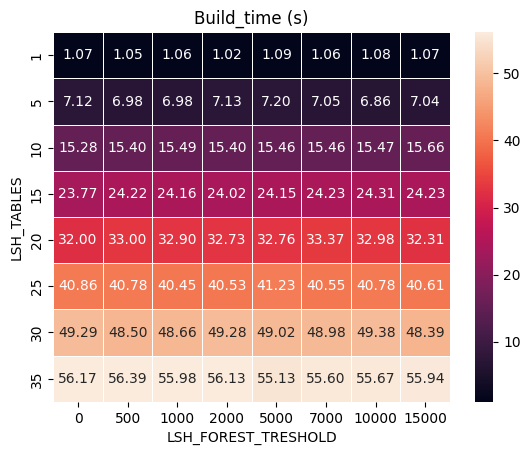
\includegraphics[width=.8\linewidth]{img/build_time.png}
      \caption{Building time della LSH generale}
      \label{fig:build_time}
    \end{subfigure}%
    \begin{subfigure}{.5\textwidth}
      \centering
      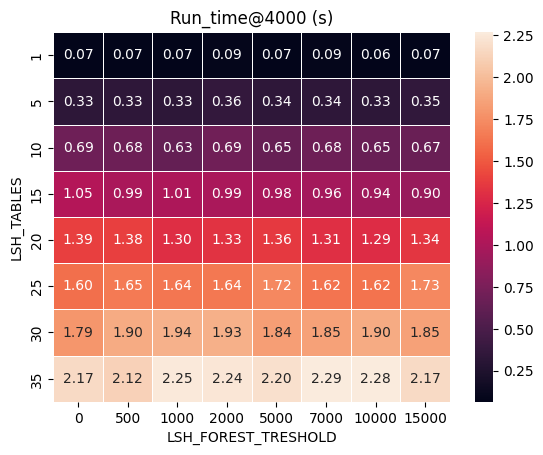
\includegraphics[width=.8\linewidth]{img/run_time.png}
      \caption{Run time}
      \label{fig:run_time}
    \end{subfigure}
    \begin{subfigure}{.5\textwidth}
      \centering
      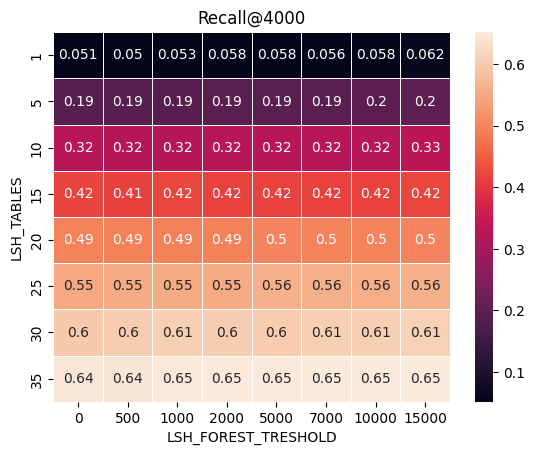
\includegraphics[width=.8\linewidth]{img/recall.png}
      \caption{Recall@4000}
      \label{fig:recall}
    \end{subfigure}
    \caption{Analisi di sensitività dei parametri, i tempi di costruzione non 
    variano al variare di LSH\_FOREST\_THRESHOLD dal momento che viene solo tracciato 
    il tempo di costruzione della LSH generale.}
    \label{fig:sensitivity}
\end{figure}

Dal momento che la Recall e il run time non vengono impattate notevolmente dal
parametro LSH\_FOREST\_THRESHOLD, risulta insignificativo evitare di creare una 
LSH dedicata per categoria. Nella soluzione consegnata è stato settato il 
parametro a $2000$.

Al contrario il parametro LSH\_TABLES è stato deciso in base ai vincoli di tempo 
richiesti dalla challenge, è stato scelto il valore $20$, ovvero il valore con la 
recall maggiore che permettesse di rispettare i vincoli di tempo. 




\section{Considerazioni}
LSH Forest è stato l'unico metodo che ci ha permesso di produrre una soluzione 
conforme ai limiti di $20$ minuti della challenge con recall maggiore rispetto
agli altri metodi ($\sim 0.4983$ sulla piattaforma di consegna). 

La motivazione per cui la recall è così bassa è dovuta principalmente dalla suddivisione 
dello spazio geometrico e dalla ricerca. Attualmente si effettuano $20$ suddisioni
dello spazio che non sono sufficientemente differenti, questo significa che in 
fase di ricerca, i bucket di ogni suddivisione in cui cade la query non hanno molta 
variabilità.

Si potrebbe migliorare questo aspetto andando cambiare il metodo di generazione 
degli iperpiani, in modo tale che ogni suddivisione dello spazio sia il più differente 
possibile, permettendo quindi di esplorare uno spazio più ampio di vettori 
sempre idealmente vicini alla query e riducendo il calcolo di distanze 
calcolate già in altre suddivisioni. 

\chapter{Soluzione vincente}
La soluzione vincente si basa su grafi metrici.

Più precisamente crea una struttura di indicizzazione a grafo ibrida, questa struttura 
è composta da un insieme di grafi HNSW, ciascuno contenente un insieme di vettori 
sufficientemente grande con metadati comuni. Ad esempio: crea un HNSW per ogni singola 
categoria sufficientemente grande e un HNSW per intervallo di timestamp.

\section{HNSW}
Hierarchical Navigable Small World Graphs (HNSW) è una struttura dati basata su 
grafi metrici a livelli che permette di navigare
lo spazio dei vettori attravero un cammino composto da archi che collegano due nodi 
vicini. Ogni livello è una 
rappresentazione dello spazio gentrico tramite un grafo metrico. Nel grafo ogni nodo rappresenta 
un vettore e si hanno degli archi diretti che rappresentano la relazione di vicinanza,
ovvero, dato un nodo ogni suo arco uscente porta ai $M$ nodi più vicini a quel nodo. La relazione 
di vicinanza è diretta perché nel caso dell'arco $(a,b)$, non è detto che il nodo 
$b$ abbia nei $M$ nodi più vicini il nodo $a$.

Ogni livello rappresenta il livello di approssimazione dello spazio geometrico, 
più il livello è alto allora maggiore è l'approssimazione, più il livello è basso 
e più precisa sarà la rappresentazione dello spazio. Dato un livello $l$, il livello 
successivo $l-1$ è un grafo composto da almeno gli stessi nodi del grafo sul livello 
precedente con l'aggiunta di nuovi nodi collegati ai nodi già presenti secondo 
la relazione di vicinanza (nel nostro caso si basa sulla distanza euclidea). Vedi 
figura \ref{fig:hnsw} 

Questo permette di navigare lo spazio velocemente nel livello più alto non passando 
per tutti i punti perché ogni nodo di un livello rappresenta una \textbf{Voronoi Cell} dello spazio grande 
quanto la specificità del livello stesso. Nodi presenti in un grafo di livello 
superiore rappresenteranno delle Voronoi Cell più grandi rispetto ai nodi 
presenti in un grafo di un livello inferiore.

\begin{figure}
    \centering
    \includegraphics*[width=0.5\textwidth]{img/hnsw.png}
    \caption{Esempio grafico di un HNSW a $3$ livelli. Il percorso con le frecce blu corrisponde 
    al percorso compiuto per cercare il nodo giallo nella struttura. 
    Il livello $0$ rappresenta l'intero spazio metrico, mentre i livelli superiori sono delle 
    approssimazioni. \cite{hnsw}}
    \label{fig:hnsw}
\end{figure}

\subsection{Creazione di HNSW}

Dato un insieme di vettori $V$, la costruzione di un generico HNSW  è un processo 
iterativo, in cui si inserisce ciascun vettore uno alla volta. L'inserimento di 
un vettore $q\in V$ nella struttura si articola nelle seguenti fasi:
\begin{itemize}
    \item \textbf{inizializzazione}: si seglie un nodo $ep$ di entry point nel livello massimo
    e si seleziona il livello $l$ a partire dal quale si inserice il vettore $q$.
    Più precisamente $l = \lfloor-\ln (U[0,1])\cdot m_l\rfloor$  e si inserirà $q$ 
    in tutti i livelli da $l$ a $0$. $m_l$ è la costante di normalizzazione che 
    limita $l\in [0, L_{max}]$, dove $L_{max}$ è il livello massimo della struttura.
    \begin{figure}
        \centering
        \includegraphics*[width=0.5\textwidth]{img/exp_decay_distr.png}
        \caption{Andamento di una funzione di densità di decadimento esponenziale. 
        \cite{exp_decay}}
        \label{fig:exp_decay}
    \end{figure}
    \item \textbf{prima fase}: a partire dal livello $L_{max}$, si naviga il grafo 
    a partire dal nodo $ep$ fino a quando non si trova il nodo $w$ più vicino a
    $q$ (algoritmo greedy), successivamente si effettua la stessa operazione 
    su livello $L_{max} - 1$, utilizzando come nodo di entry point il nodo $w$,
    si itera il procedimento fino a quando non si trova l'entry point $w$ del livello $l$.
    \item \textbf{seconda fase}: a partire dal livello $l$ si cercano i $W$ nodi 
    più vicini a $q$ a partire dall'ultimo entry point trovato al termine della fase precedente ($|W| = efConstruction$),
    sempre col medesimo algoritmo greedy accennato nella prima fase.
    Successivamente si usa un'euristica che calcola dall'insieme dei $W$ nodi
    l'insieme $N$ degli $M$ nodi più vicini a $q$ sempre sullo stesso layer $l$. 
    Si creano degli edge bidirezionali tra i nodi $N$ e $q$. Successivamente si 
    sistemano i collegamenti tra i vicini in modo che ogni nodo rispetti il vincolo 
    di avere al massimo $M_{max}$ collegamenti, questo viene implementato rimuovendo 
    degli edge tra due nodi nel vicinato di $q$. Infine si reitera il procedimento 
    dal livello $l$ al livello $0$.
\end{itemize}

\begin{nota}
    La scelta del livello dal quale inserire un nuovo vettore viene effettuata 
    in modo randomico secondo una \textbf{distribuzione di decadimento esponenziale}. 
    In sostanza si ha maggior probabilità di estrarre un livello $l$ vicino a $0$ 
    piuttosto che un livello più vicino a $L_{max}$. (vedi figura \cite{exp_decay})
\end{nota}

\begin{nota}
    L'algoritmo greedy accennato precedentemente permette di navigare il grafo 
    ad un particolare livello a partire da un nodo di entrypoint $ep$ e trovare gli $ef$ 
    nodi candidati vicini al vettore $q$. 
    La ricerca avviene nel seguente modo:
    \begin{itemize}
        \item si tiene traccia dei nodi già visitati, dei nodi vicini a $q$. Inizialimente 
        entrambi gli insiemi sono vuoti.
        \item si parte dal nodo $ep$, si aggiunge $ep$ all'insieme dei nodi vicini a $q$,
        si guardano tutti i vicini e si calcola la distanza da ciascun vicino a $q$,
        si sceglie il vicino a distanza minima e ci si sposta in quel nodo, si 
        aggiunge $ep$ all'insieme dei nodi visitati.
        \item si reitera il punto precedente, evitando di visitare nodi già visitati e
        fino a quando non si può più andare avanti, oppure si continua fino a quando 
        non si arriva ad una iterazione massima. Se l'insieme dei vicini a $q$
        superla $ef$ allora vengono rimossi i nodi più lontani da $q$.
    \end{itemize} 
\end{nota}

Per la costruzione della struttura si richiedono i seguenti parametri:
\begin{itemize}
    \item $M_{max}$: numero massimo di edge uscenti da ogni nodo per un livello, questo 
    potrebbe coincidere con $M$.
    \item $L_{max}$: livello massimo della struttura.
    \item $efConstruction$: specifica il numero dei nodi candidati ad essere i vicini 
    del vettore $q$. Questo parametro permette di variare la recall e il tempo di 
    costruzione della struttura.
\end{itemize} 



\subsection{Ricerca nella struttura}
La ricerca di una query $q$ in un generico HNSW richiede i seguenti parametri:
\begin{itemize}
    \item $K$: numero di vicini alla query $q$ da cercare nella struttura
    \item $ef$: numero di candidati vicini da considerare quando si naviga sui singoli 
    grafi di ciascun livello.
\end{itemize}

La ricerca si articola nei seguenti passi:
\begin{itemize}
    \item si sceglie randomicamente un entry point $ep$ nel livello massimo
    \item nel livello massimo si cercano gli $ef$ migliori vicini alla query 
    $q$ mediante l'algoritmo greedy di graph traversal usato in fase di costruzione
    \item si estrae dai migliori $ef$ vicini alla query il più vicino e lo si usa 
    come $ep$ per il grafo al livello inferiore.
    \item si reitera il procedimento fino a quando non si ottengono gli $ef$ vicini 
    alla query al livello $0$. In questo caso si ritornano i migliori $K$ vicini.
\end{itemize}  

\section{Creazione della struttura di indicizzazione}
Per prima cosa vene letto tutto il dataset e viene salvato
all'interno di $3$ array:
\begin{itemize}
    \item \texttt{base\_vecs}: array contenente i coefficienti di tutti i vettori del dataset
    di dimensione $10^7\cdot 100$.
    \item \texttt{base\_labels}: array contente le labels di tutti i vettori, ovvero un 
    vettore di $10^7$ elementi.
\end{itemize} 

\begin{nota}
    La posizione $i$ indica  l'informazione dell'$i$-esimo vettore nel dataset.
\end{nota}

Successivamente si creano degli array di appoggio che specificano l'ordinamento 
del dataset rispetto a diversi criteri di ordinamento:
\begin{itemize}
    \item \texttt{sorted\_base\_ids}: vettore contenente gli indici dei vettori ordinati 
    per categoria crescente e successivamente per timestamps. Quindi per ogni $i\le j\in \mathbb{N}$,
    allora il numero della categoria associato al vettore $sorted\_base\_ids[i]$
    è minore rispetto al numero della categoria del vettore $sorted\_base\_ids[j]$,
    in caso di categorie uguali allora si ordina per timestamps.
    \item \texttt{sorted\_base\_ids\_by\_time}: vettore contenente gli indici dei vettori ordinati 
    per timestamps spostando i spostando tutti i vettori della categoria più grande all'inizio 
    del vettore. In questo modo all'inizio del vettore si avranno solo vettori 
    ordinati per timestamps della categoria più grande, successivamente si hanno 
    tutti gli altri vettori ordinati per timestamp. 
    \item \texttt{sorted\_base\_ids\_by\_full\_time}: vettore contenente gli indici dei vettori ordinati 
    per timestamps.
\end{itemize}

\begin{nota}
    L'ordinamento dei vettori della categoria più grande in sorted\_base\_ids\_by\_time 
    viene replicato dal vettore sorted\_base\_ids perché in caso ci fossero vettori 
    della categoria più grande con lo stesso timestap allora questi possono avere 
    un ordinamento diverso tra i due indici.
\end{nota}

In aggiunta viene creata una $c\_map$, ovvero una mappa delle categorie ovvero 
un array di coppie ordinate:
\begin{equation}
    category\_map[c] = \langle i, dimensione\_categoria\_c\rangle
\end{equation} 
dove $i = sorted\_base\_ids[v]$ con $v$ ultimo vettore della categoria $c$, 
mentre $dimensione\_categoria\_c$ specifica il numero di vettori presenti nella 
categoria $c$. Da notare che la coppia viene aggiunta all'array solo quando $c$ 
ha almeno $450000$ vettori.

Successivamente si costruisce una $t\_map$, ovvero una mappa dei timestamp ovvero 
un array di coppie ordinate:
\begin{equation}
    t\_map[i] = \langle l, dimensione\_intervallo\rangle
\end{equation} 
dove:
\begin{itemize}
    \item $i\in \{0,\dots,9\}$ specifica l'intervallo di timestamp $[0.1*i, 0.1*(i+1)]$
    \item $l= timestamps\_by\_full\_time[v]$, $v$ è il primo vettore con il timestamp nell'intervallo cercato
    \item $dimensione\_intervallo$ il numero di vettori nell'intervallo
\end{itemize}

In seguito viene letto il query set e viene salvato all'interno di due array:
\begin{itemize}
    \item \texttt{query\_vecs}: array contente le componenti dei vettori di query ovvero 
    $10^6 \cdot 100$.
    \item \texttt{query\_metas}: array contente i metadati delle query, ovvero la tipologia,
    la categoria e l'intervallo di timestamp.
    $10^6 \cdot 4$.
\end{itemize}

Successivamente si creano degli array di appoggio:
\begin{itemize}
    \item \texttt{sorted\_ids}: vettore degli indici dei delle query ordinate per tipo, 
    categoria, lower bound e upper bound dell'intervallo di timestamp
    \item \texttt{category\_query}: mappa che associa per ogni categoria un vettore di 
    indici di query che afferiscono a quella categoria.
\end{itemize}

Da notare che la $c\_map$, $category\_query$ e $t\_map$ sono tutte mappe implementate 
come \texttt{unordered\_map}.

Dopo la lettura ordinata del dataset e del queryset, è stato applicato un passo di 
\textbf{quantizzazione scalare simmetrica} in modo da ridurre lo spazio occupato dalle componenti, 
più precisamente si riduce da $400B$ a $112B$, trasformando tutte le combonenti in 
un byte. Ogni vettore occupa $112B$ perché $100B$ sono per le $100$ componenti mentre i restanti $12B$
sono posti a zero e servono ad un duplice scopo: avere un'allineamento a $32bits$/$64bits$ per questioni
di indirizzamento (altrimenti non ci sono assicurazioni su come compilatore intende allineare la memoria),
e avere contemporaneamente un allineamento a $16B$ per poter sfruttare le operazioni del \textbf{SSE} (estensione SIMD
che permette di operare in parallelo su registri a $128bits$).

In senguito è stato creato un HSNW per i vettori 
afferenti alla categoria più grande, uno per i vettori afferenti a categorie che 
contengono almento $500000$ vettori e uno per ogni intervallo di timestamp della 
$t\_map$. Gli HNSW vengono costruiti sulle codifiche dei vettori.

In aggiunta, vengono calcolate tutte le codifiche della quantizzazione scalare 
di tutti i vettori del dataset. Inoltre, si creano due vettori di ordinamento 
che specificano l'ordinamento delle condifiche:
\begin{itemize}
    \item \texttt{sorted\_both}: in posizione $i$ contiene i metadati dell'$i$-esima
    codifica dei vettori del dataset secondo l'ordinamento per categoria e successivamente
    per timestamp.
    \item \texttt{sorted\_timestamp}: in posizione $i$ contiene i metadati dell'$i$-esima
    codifica dei vettori del dataset secondo l'ordinamento per timestamp.
\end{itemize}

%La struttura di indicizzazione definita dagli autori è composta da:
%\begin{itemize}
%    \item \texttt{base\_vecs}
%    \item \texttt{base\_labels}
%    \item \texttt{sorted\_base\_ids}
%    \item \texttt{sorted\_base\_ids\_by\_time} 
%    \item \texttt{sorted\_base\_ids\_by\_full\_time}
%    \item \texttt{sorted\_both}
%    \item \texttt{sorted\_timestamp}
%    \item \texttt{c\_map}
%    \item \texttt{t\_map}
%    \item un grafo HNSW per la categoria più grande.
%    \item un grafo HNSW per ogni categoria più grande di $500000$ vettori.
%    \item un grafo HNSW per ogni intervallo di timestamp, in totale $10$.
%\end{itemize}

\subsection{Implementazione di HNSW}

\paragraph{Configurazione}

Vengono costruiti un grafo HNSW per la categoria $C_b$ pi\`u grande, uno per ogni categoria $C_i \ne C_b$ con $|C_i| > 500000$ e infine uno per ogni intervallo di timestamp nella $t\_map$.
I parametri di costruzione degli HNSW specificati dagli autori sono $M = 28$ e $efConstruction = 200$.
In generale il numero di massimo di layer ottenibili nell'HNSW scala come $\frac 1 {ln(M)}$, ovvero con una probabilit\`a molto piccola (si richiama la sezione d'introduzione su HNSW: la frazione \`e moltiplicata per una variabile uniforme $x \; : \; [0,1]$) verr\`a estratto un layer superiore allo zero. Con questa configurazione di parametri ci si pu\`o aspettare asintoticamente un numero molto basso di layer.

\paragraph{Il Wrapper}

Gli autori della soluzione hanno sfruttato l'implementazione di HNSW della libreria \href{https://github.com/zilliztech/pyglass/tree/master}{pyglass} creando un wrapper per le strutture definite dalla libreria.
Questo wrapper applica una quantizzazione scalare simmetrica a $8$ bit (descritta precedentemente) per sfruttare le operazioni vettoriali del processore, velocizzando il calcolo delle distanze.
Quindi aggiunge i punti sequenzialmente ma sfruttando la parallelizzazione: questo grazie alla presenza e uso di lock all'interno dell'implementazione dell'HNSW di \textit{pyglass}.
Il primo punto inserito \`e per\`o escluso dalla parallelizzazione, altrimenti eseguendo in parallelo verrebbero aggiungiunti fino a 32 nodi come entry point.
Dopo aver inserito tutti i dati, il wrapper costruisce un grafo che copia sostanzialmente il Layer 0 dell'HNSW, tracciando oltre agli indici dei nodi puntati dagli archi il timestamp di ogni nodo bersaglio.
Questo grafo contiene anche un \textbf{Initializer} utilizzato in fase di ricerca per inizializzare il pool di candidati nodi vicini.

\paragraph{La Libreria}

L'algoritmo di inserimento dei punti implementato dalla libreria ricalca essenzialmente gli algoritmi presentati nella sezione precedente e presentati dal paper ufficiale di HNSW, tuttavia applica una serie di ottimizzazioni che lo rendono pi\`u veloce di una implementazione naive.

Per cominciare, la fase iniziale di ricerca per l'entry point pi\`u vicino viene effettuata tramite una variante della ricerca su Layer che non tiene traccia di tutti i nodi identificati e che sono candidati ma solo del pi\`u vicino, quindi ogni iterazione all'interno di un livello tiene conto solo dell'euristicamente "migliore" vicino.
Questo ha l'effetto di velocizzare quella fase a discapito della previsione, ragion per cui nella fase successiva si tiene traccia di una coda di candidati per evitare di perdere informazioni.

Nella funzione di ricerca su layer vera e propria invece tra gli accorgimenti troviamo delle istruzioni Streaming SIMD Extension che permettono all'hardware di precaricare le pagine con i dati da usare nella Cache, il che velocizza i tempi di accesso in maniera sensibile.
Inoltre nella fase di aggiornamento dei collegamenti in un layer si ritarda l'inserimento dell'arco inverso dal vicino i-esimo al punto che si sta inserendo e si sfrutta l'euristica di selezione di migliori M vicini dalla lista dei candidati (in questo caso il vicinato del vicino e il punto in inserimento).

Infine il fatto di inserire parallelamente i punti permette ad ogni sottoricerca di considerare meno punti e questo snellisce di poco l'aggiunta di nuovi nodi al grafo.

\section{Ricerca nella struttura di indicizzazione}

La ricerca nella struttura a grafo ibrida ha diverse strategie in base alle singole 
query. In generale si effettua una ricerca sfruttando le codifiche dei vettori, 
in questo caso si estrae un insieme di vettori maggiore rispetto a quelli richiesti 
dalla challenge, in generale almeno $140$. Poi in un secondo momento si raffina 
il risultato andando ad estrare dai questi $140$ i migliori $100$ usando la loro 
rappresentazione nello spazio originale non quantizzato. 

La prima operazione della ricerca si basa sull'ordinamento di tutte le query 
secondo due criteri differenti:
\begin{itemize}
    \item il primo per le label e poi per timestamp
    \item il secondo per timestamp
\end{itemize} 
Successivamente per ogni query viene calcolata la sua codifica usando la quantizzazione 
scalare sui coefficienti del vettore di query.

In seguito, viene calcolata la selettività di ciascuna query, per selettività
si intende il numero totale di vettori candidati ad essere potenziali vicini alla 
query rispetto i parametri di ricerca sui metadati. 
La selettività viene calcolata in tempo costante confrontando solo i metadati in 
base alla tipologia di query, sfruttando la $c\_map$ e la $t\_map$. 

La selettività di una query determina, insieme ai metadati della query, la strategia 
da adottare in fase di ricerca.

La \textbf{prima strategia} di ricerca è nel caso in cui la query è di tipo $1,2,3$ 
e la sua selettività è inferiore rispettivamente a $500000$, per i primi due, e $800000$, 
per l'ultimo tipo di query. In questo caso 
si effettua una ricerca esaustiva sfruttando le codifiche dei vettori candidati 
e gli array di ordinamento delle codifiche (\texttt{sorted\_both} e \texttt{sorted\_timestamp}).
Durante la ricerca si estraggono $140$ vettori vicini al vettore di query nello 
spazio delle condifiche e infine, di questi vettori, si scelgono $100$ vettori 
più vicini alla query nello spazio originale. 

La \textbf{seconda strategia} di ricerca è per le query di tipo $1$ che ha una selettività 
maggiore di $500000$ vettori. In questo caso la ricerca si effettua nel grafo 
HNSW della stessa categoria del metadato della query. I parametri di ricerca nell'HNSW
sono i seguenti 
$$K = 140 \qquad M= \lceil1800+(700)/(maxc\_size - minc\_size)dim\_cat\rceil$$
Dove:
\begin{itemize}
    \item $maxc\_size$: è la dimensione della categoria più grande presente 
    nel dataset.
    \item $minc\_size$: dimensione della categoria più piccola presente.
    nel dataset
    \item $dim\_cat$: dimensione della categoria in cui afferisce la query.
\end{itemize}
Dal risultato estratto dal grafo si effettua un raffinamento andando ad estrarre 
i $100$ migliori vettori nello spazio originale.

La \textbf{terza strategia} di ricerca è per le query di tipo $3$ che ha una selettività 
maggiore di $800000$ vettori. In questo caso la strategia è identica alla seconda 
ma con i seguenti parametri di ricerca nell'HNSW.(\textbf{RICERCA FILTRATA (OVVIAMENTE NON SI CAPISCE NULLA)}) 
$$K = 150 \qquad M= \lceil1800+(1000)/(maxc\_size - minc\_size)dim\_cat\rceil$$

La \textbf{quarta strategia} di ricerca è per le query di tipo $0$. In questo caso 
si effettua una ricerca parallela nei $10$ HNSW dei sotto-intervalli di timestamp 
usando per ognuna i seguenti parametri:
$$M=450 \qquad K=150$$
In questo modo si ottengono $150\cdot 10$ vicini alla query nello spazio delle 
codifiche, successivamente si raffinano i risultati estraendo i migliori $100$ 
vettori rispetto allo spazio originale.

La \textbf{quinta strategia} di ricerca è per la query di tipo $2$ che ha una 
superiore a $500000$. In questa strategia si sfruttano gli HNSW creati per i $10$
sottointervalli di timestamp, più precisamente si controlla la copertura dell'intervallo 
$[l,r]$ della query rispetto ai sottointervalli $[l',r']$ e se $[l,r]\cap [l',r']$ 
allora si ricerca nell'HNSW del sottointervallo $[l',r']$. 
In particolare in base alla selettività della query variano i parametri di ricerca:
\begin{itemize}
    \item se la query ha una selettività inferiore a $2000000$ di vettori, allora 
    per un generico sottointervallo $[l',r']$ abbiamo le seguenti casistiche:
    \begin{itemize}
        \item $[l,r]\cap [l',r'] = \emptyset$: si ignora il sottointervallo perché 
        l'HNSW contiene solo vettori in $[l',r']$ che sono fuori dall'intervallo 
        di query.
        \item $[l,r] = [l',r'] \lor  [l',r'] \subseteq [l,r]$: tutti i vettori 
        del sottointervallo solo potenziali candidati, quindi si effettua una ricerca nell'HNSW
        utilizzando parametri $M=780$ e $K=150$.
        \item $[l',r'] \cap [l,r] \ne \emptyset, [l',r'] \not \subseteq [l,r]$: 
        solo una parte dei vettori sono dei potenziali candidati, quindi in base 
        all'ampiezza di $[l',r'] \cap [l,r]$ si hanno diverse strategie:
        \begin{itemize}
            \item se l'intersezione è inferiore al $50\%$ di $[l',r']$ allora si effettua una 
            ricerca esaustiva delle $150$ codifiche più vicine alla codifica del 
            vettore di query. Per fare ciò si sfrutta la $t_map$ e 
            l'ordinamento delle codifiche rispetto il timestamp.
            \item se l'intersezione è superiore al $50\%$ di $[l',r']$ allora si effettua una 
            ricerca nell'HNSW del sottointervallo $[l',r']$ con i parametri $M=1180$ e $K=150$.
        \end{itemize}
    \end{itemize}
    \item se la query ha una selettività superiore a $2000000$ di vettori, allora 
    per un generico sottointervallo $[l',r']$ abbiamo le stesse casistiche 
    del caso con selettività inferiore a $2000000$, con la differenza che cambia
    la soglia per la ricerca esaustiva e i parametri della ricerca nel grafo. Più 
    precisamente:
    \begin{itemize}
        \item se $[l',r'] \not \subseteq [l,r]$ allora si ignora il sottointervallo.
        \item se $[l,r] = [l',r'] \lor  [l',r'] \subseteq [l,r]$:
        \begin{itemize}
            \item se la query seleziona fino a $3000000$ vettori allora ricerca 
            nell'HNSW di $[l',r']$ con $K=150$ e $M=1180$
            \item se la query seleziona da $3000000$ a $6000000$ vettori allora ricerca 
            nell'HNSW di $[l',r']$ con $K=150$ e $M=780$
            \item se la query seleziona sopra $6000000$ vettori allora ricerca 
            nell'HNSW di $[l',r']$ con $K=150$ e $M=680$
        \end{itemize}
        \item se $[l',r'] \cap [l,r] \ne \emptyset, [l',r'] \not \subseteq [l,r]$:
        \begin{itemize}
            \item se la query seleziona fino a $3000000$ vettori allora ricerca 
            nell'HNSW di $[l',r']$ con $K=150$ e $M=780$
            \item se la query seleziona da $3000000$ a $6000000$ vettori allora ricerca 
            nell'HNSW di $[l',r']$ con $K=150$ e $M=680$
            \item se la query seleziona sopra $6000000$ vettori allora ricerca 
            nell'HNSW di $[l',r']$ con $K=150$ e $M=480$
        \end{itemize}
    \end{itemize}
\end{itemize}

Quindi alla fine si producono un totale di $150$ vettori per ogni sottointervallo
$[l',r']$ con intersezione non nulla con l'intervallo di query e, in conclusione, 
si raffina il risultato estraendo i migliori $100$ vettori più vicini alla query 
nello spazio originale.   

\subsection{Considerazioni sulla ricerca}

Dal momento che sono state definite diverse strategie di ricerca, questo rende 
complicato la sua analisi di complessità di ricerca di una query.

L'osservazione più naturale che nasce dopo aver visto per la prima volta la ricerca,
è che la quantizzazione è l'elemento chiave. Infatti, calcolare la distanza sugli 
elementi quantizzazioni risulta nettamente più efficiente rispetto a calcolare la 
distanza sugli elementi, questo permette quindi agli autori di effettuare ricerche 
esaustive su numerosi elementi, cosa che noi non potevamo permetterci di fare.

Inoltre, la ricerca consiste alla fine nell'effettuare una ricerca esausiva 
oppure nell'effettuare una ricerca nell'HNSW. In generale la ricerca esaustiva è 
lineare ma limitata a massimo $1000000$ di vettori (nel caso della ricerca di una 
query di tipo 2), difficile che possa capitare dal momento che sarebbero tutti 
all'interno di un sottointervallo. Al contrario la ricerca nell'HNSW si effettua 
in tempo logaritmico e questo permette di velocizzare le ricerche per query ad 
alta selettività. 


% si articola nelle seguenti fasi:
% \begin{itemize}
%     \item codifica tutti i vettori, definisce due ordinamenti delle codifiche:
%     \begin{itemize}
%         \item il primo che ordina per label e timestamp
%         \item il secondo che ordina per timestamp
%     \end{itemize}
%     \item calcola le codifiche di tutte le query per calcolare le distanze in modo 
%     più efficiente.
%     \item si calcola la selettività di ciascuna query del tipo $1,2,3$, ovvero 
%     si calcolano il numero totale di candidati che rispettano i criteri di filtraggio 
%     per ciascuna query. Questo è stato implementato in tempo costante mediante la 
%     $t\_map$, la $c\_map$ e i due ordinamenti dei vettori effettuati in precedenza rispetto 
%     la categoria e rispetto il timestamp. 
%     \item se la query di tipo $1,2$ seleziona un numero di vettori 
%     inferiore a $500000$ o se la query di tipo $3$ seleziona un numero di vettori 
%     inferiore a $800000$ allora si effettua una ricerca esaustiva usando le codifiche 
%     dei vettori e la codifica della query. In questo modo si estraggono le $140$
%     migliori codifiche più vicine alla codifica della query (usando la distanza 
%     calcolata sulle codifiche) e si selezionano, tra queste $140$, i migliori $100$
%     vettori più vicini alla query usando la loro rappresentazione nativa e quindi 
%     calcolando le distanze sulle versioni di dimensione $100$.
%     \item se la query di tipo $1$ seleziona un numero di vettori 
%     superiore a $500000$ o se la query di tipo $3$ seleziona un numero di vettori 
%     superiore a $800000$ allora si effettua una ricerca nel grafo metrico HNSW 
%     dedicato alla categoria della query. I parametri della ricerca nell'HNSW sono
%     rispettivamente:
%     \begin{itemize}
%         \item per la query di tipo $1$: cerca un totale di $K=140$ vettori considerando 
%         un totale $M= \lceil1800+(700)/(maxc\_size - minc\_size)dim\_cat\rceil$ 
%         nodi vicini durante la ricerca. Dove $maxc\_size$ è la dimensione della categoria 
%         più grande presente 
%         nel dataset, $minc\_size$ dimensione della categoria più piccola presente 
%         nel dataset e $dim\_cat$ dimensione della categoria in cui afferisce la query.
%         \item per la query di tipo $3$: cerca un totale di $K=140$ vettori considerando 
%         un totale $M= \lceil1800+(1000)/(maxc\_size - minc\_size)dim\_cat\rceil$ 
%         nodi vicini durante la ricerca (le variabili per $M$ sono le stesse introdotte 
%         al punto precedente).  (\textbf{RICERCA FILTRATA (OVVIAMENTE NON SI CAPISCE NULLA)})
%     \end{itemize} 
%     Infine una volta ottenuti i migliori $140$ vettori si estraggono i migliori $100$
%     più vicini usando la distanza euclidea sulla rappresentazione dello spazio 
%     originale.
%     \item se la query è di tipo $0$ allora si effettua una ricerca parallela nei 
%     $10$ HNSW dei sotto-intervalli di timestamp usando per ognuna i seguenti parametri:
%     \begin{itemize}
%         \item $M=450$
%         \item $K=140$
%     \end{itemize} 
%     Infine si ottengono i migliori $100$ vettori nello spazio originale che sono 
%     a distanza minima rispetto ai totali $140\cdot 10$ vettori candidati.
%     \item se la query è di tipo $2$ e seleziona un numero di vettori 
%     superiore a $500000$ allora si applica una stategia di ricerca in base alla 
%     copertura dell'intervallo di timpestamp della query $[l,r]$ rispetto ai $10$ sottointervalli
%     di timestamp indicizzati. Più precisamente:
%     \begin{itemize}
%         \item se la query seleziona meno di $2000000$ di vettori allora per un 
%         generico sottointervallo $[l',r']$ di timestamp indicizzato:
%         \begin{itemize}
%             \item se $[l,r]$ non copre $[l',r']$ allora si ignora il sottointervallo.
%             \item se $[l,r] = [l',r'] \lor  [l',r'] \subseteq [l,r]$ allora 
%             tutti i vettori del sottointervallo solo potenziali candidati, 
%             quindi si effettua una ricerca nell'HNSW
%             utilizzando parametri $M=780$ e $K=150$.
%             Infine dei $150$ vicini alla query estratti, si scelgono i migliori $100$ 
%             nello spazio originale.
%             \item se $[l',r'] \cap [l,r] \ne \emptyset, [l',r'] \not \subseteq [l,r]$ 
%             allora si hanno diverse strategie in base alla percentuale di vettori in $[l',r']$ 
%             selezionati dalla query:
%             \begin{itemize}
%                 \item se in $[l',r']$ la query seleziona fino al $50\%$ dei vettori,
%                 si effettua una ricerca esaustiva delle $140$ migliori codifiche 
%                 più vicine alla codifica della query nella regione $[l,r] \cap [l',r']$.
%                 \item se in $[l',r']$ la query seleziona almeno $50\%$ dei vettori,
%                 si ricerca nell'HNSW con parametri $M=1180$ e $K=140$
%             \end{itemize} 
%         \end{itemize}
%         \item se la query seleziona almeno $2000000$ allora:
%         \begin{itemize}
%             \item se $[l',r'] \not \subseteq [l,r]$ allora si ignora il sottointervallo.
%             \item se $[l,r] = [l',r'] \lor  [l',r'] \subseteq [l,r]$ allora 
%             tutti i vettori del sottointervallo solo potenziali candidati e si 
%             hanno diverse strategie in base al numero di vettori selezionati nel 
%             dataset dalla query allora variano i parametri di ricerca:
%             \begin{itemize}
%                 \item se la query seleziona fino a $3000000$ allora ricerca 
%                 nell'HNSW di $[l',r']$ con $K=140$ e $M=1180$
%                 \item se la query seleziona da $3000000$ a $6000000$ allora ricerca 
%                 nell'HNSW di $[l',r']$ con $K=140$ e $M=780$
%                 \item se la query seleziona sopra $6000000$ allora ricerca 
%                 nell'HNSW di $[l',r']$ con $K=140$ e $M=680$
%             \end{itemize}
%             Infine dei $140$ vicini alla query estratti, si scelgono i migliori $100$ 
%             nello spazio originale.
%             \item se $[l',r'] \cap [l,r] \ne \emptyset, [l',r'] \not \subseteq [l,r]$ 
%             allora si hanno diverse strategie sempre in base al numero di vettori 
%             selezionati dalla query nel dataset:
%             \begin{itemize}
%                 \item se la query seleziona fino a $3000000$ allora ricerca 
%                 nell'HNSW di $[l',r']$ con $K=140$ e $M=780$
%                 \item se la query seleziona da $3000000$ a $6000000$ allora ricerca 
%                 nell'HNSW di $[l',r']$ con $K=140$ e $M=680$
%                 \item se la query seleziona sopra $6000000$ allora ricerca 
%                 nell'HNSW di $[l',r']$ con $K=140$ e $M=480$
%             \end{itemize}
%         \end{itemize}
%     \end{itemize} 
%     Quindi per ogni query che specifica un filtraggio sull'intervallo $[l,r]$ allora 
%     si scompone l'intervallo in tanti sottointervalli $[l',r']_i$ contigui dai quali 
%     si estraggono per ognuno $140$ vettori migliori secondo le codifiche, infine 
%     si aggregano e si prendono solo i $100$ migliori. 
% \end{itemize}




% - selezionata i vettori codificati in base alla tipologia di query
% - se < 500000 oppure query tipo 3 < 800000 allora fa bruteforce e ricerca le migliori $140$ codifiche a $112 B$
% più vicine a quella di query e poi seleziona le $100$ migliori rispetto ai valori 
% nativi
% - per tipo 1 > 500000 e tipo 3 > 800000  effetua una ricerca in HNSW $K= \lceil1800+(2500-1800)/(maxc_size - minc_size)dim_cat\rceil$
%  $K= \lceil1800+(2800-1800)/(maxc_size - minc_size)dim_cat\rceil$
%  Seleziona i migliori $150$ vettori che rispettano il filtro, infine estraggo i 
%  migliori $100$.

% - per tipo 0 oltre alla ricerca in brute force, ricerca nei grafi dei timestamp.
%  Più precisamente si ottengono $150$ candidati per ciascuna query dalla ricerca 
%  parallela nei grafi di ciascun timestamp. Più precisamente per ciascun grafo di 
%  timestamp si cercano $450$ vicini alla query, dai quali si estraggono solo i primi 
%  $150$ per ogni grafo e, infine, si aggregano i risultati in un pool 
%  di candidati per ogni query grande $150$ vettori preferendo sempre i più vicini.
%  (nota nella parte di bruteforce cerca un solo vicino, forse è un errore che hanno 
%  lasciato)

%  Avendo $10$ sottointervalli di timestamp si ottengono un totale di $150*10$ candidati 
%  e si aggregano scegliendo i migliori $100$.
 
% - tipo 2: se quelli selezionati rispetto al filtro sono > 500000 e > 800000 allora 
%  seleziona la strategia di ricerca in base alla copertura di $[l,r]$ sulle $10$ 
%  suddivisioni del timestamp, data una suddivisione $[l',r']$:
%     - se il numero di vettori selezionati in precedenza è < 2000000 e $[l,r]$ copre 
%     tutto $[l',r']$ allora si cerca direttamente nel grafo metrico dell'intervallo $[l',r']$ (ricerca FULL),
%     se [l,r] copre fino ad un massimo del $50\%$ della suddivisione [l',r'] allora 
%     ricerca in bruteforce in quell'intervallo. Altrimenti fai ricerca MEDIUM
%     - se il numero di vettori selezionati in precedenza è >= 2000000 fai la stessa 
%     cosa di sopra ma abbassando la threshold di bruteforce a  $20\%$

%   Effettua la ricerca della query rispetto alle strategie definite prima:
%     - bruteforce: i migliori 140 vettori nel sottointervallo [l',r'] intersecato [l,r]
%     e li mette nel pool di candidati.
%     - MEDIUM: se l'insieme dei vettori da confrontare è < 3000000 allora si estraggono 
%     dal sottointervallo [l',r'] i vicini $1180$ dalla query, se sono in totale <= 6000000 e >=  3000000
%     allora si estraggono dal sottointervallo [l',r'] i vicini $780$ dalla query, 
%     se sono in totale > 6000000 allora si estraggono dal sottointervallo [l',r'] i vicini $680$ dalla query.
%     e di questi se ne estraggono $150$
%     - FULL: se l'insieme dei vettori da confrontare è < 3000000 allora si estraggono 
%     dal sottointervallo [l',r'] i vicini $780$ dalla query, se sono in totale <= 6000000 e >=  3000000
%     allora si estraggono dal sottointervallo [l',r'] i vicini $630$ dalla query, 
%     se sono in totale > 6000000 allora si estraggono dal sottointervallo [l',r'] i vicini $480$ dalla query.
%     e di questi se ne estraggono $150$
  
%   In questo modo se $[l,r]$ include in totale $5$ sotto intervalli contigui [l',r']
%   allora si ottengono $150*5$ e infine si scelgono i migliori $100$.


\printbibliography

\end{document}
